\section{esercizio 10}
\textit{\textbf{Descrizione:} Scaricare la function cremat che crea sistemi lineari $n \times n$ la cui soluzione \'e il vettore $v = (1 \cdots n)^{T}$. Eseguire, quindi, lo script Matlab (vedere esercizio) per testare le function dei precedenti esercizi. Confrontare i risultati ottenuti con quelli attesi, e dare una spiegazione esauriente degli stessi.}\newline
\noindent\emph{Soluzione: }
\\~\\
Una volta scaricata la funzione cremat
\\~\\

\section*{cremat}
\lstinputlisting{resources/cremat.m}

ed eseguito il seguente script
\\~\\
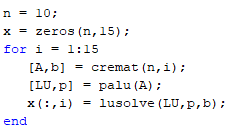
\includegraphics[width=.5\linewidth]{img/ex10.png}
\\~\\
otteniamo i seguenti risultati
\\~\\
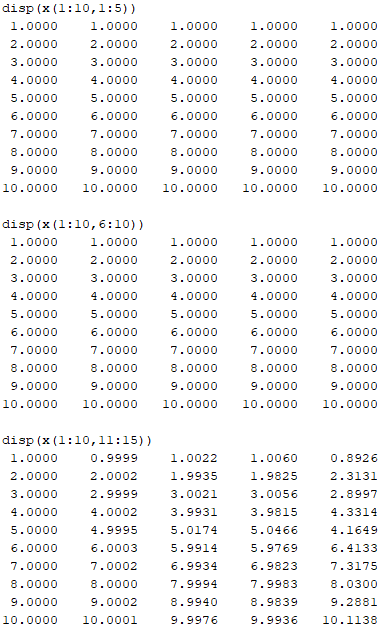
\includegraphics[width=.65\linewidth]{img/tabella10.png}\\~\\
notiamo che i risultati ottenuti coincidono con i risultati attesi per k<12, quindi abbiamo dei risultati perturbati.\newline
Questo vuol dire che per il condizionamento del problema per le matrici

\begin{equation}
	\frac{\left \| \Delta x \right \|}{\left \| x \right \|} \leq k(A)\cdot \left ( \frac{\left \| \Delta b \right \|}{\left \| b \right \|} + \frac{\left \| \Delta A \right \|}{\left \| A \right \|}\right )
\end{equation}
abbiamo un numero di condizionamento di A molto piccolo e quindi una matrice ben condizionata per $1 \leq k<12$ ed un numero di condizionamento di A $>>$ 1 e quindi una matrice mal condizionata per $k \geq 12$